% Created 2016-08-29 Mon 12:14
\documentclass[presentation]{beamer}
\usepackage[utf8]{inputenc}
\usepackage[T1]{fontenc}
\usepackage{fixltx2e}
\usepackage{graphicx}
\usepackage{grffile}
\usepackage{longtable}
\usepackage{wrapfig}
\usepackage{rotating}
\usepackage[normalem]{ulem}
\usepackage{amsmath}
\usepackage{textcomp}
\usepackage{amssymb}
\usepackage{capt-of}
\usepackage{hyperref}
\usetheme{default}
\author{Paul M. Magwene}
\date{29 August 2016}
\title{Bio 204: Biological Data Analysis}
\definecolor{links}{HTML}{2A1B81}
\hypersetup{colorlinks,linkcolor=,urlcolor=magenta}
\useinnertheme[shadow,outline]{chamfered}
\usecolortheme{beaver}
\beamertemplatenavigationsymbolsempty
\usefonttheme{professionalfonts}

\let\digamma\relax
\usepackage[scale=0.85,stdmathitalics=true,romanfamily=casual]{lucimatx}

\usepackage[scaled=0.85]{zi4}  % inconsolata font
\renewcommand*\familydefault{\ttdefault}

\usefonttheme[stillsansseriftext]{serif}


\institute[Duke]{Department of Biology}
\hypersetup{
 pdfauthor={Paul M. Magwene},
 pdftitle={Bio 204: Biological Data Analysis},
 pdfkeywords={},
 pdfsubject={},
 pdfcreator={Emacs 25.1.1 (Org mode 8.3.5)}, 
 pdflang={English}}
\begin{document}

\maketitle

\begin{frame}[label={sec:orgheadline1}]{Welcome}
\begin{itemize}
\item Introductions
\item What is ``Biological Data Analysis''?
\item Grading and course policies
\item Course Overview
\end{itemize}
\end{frame}

\begin{frame}[label={sec:orgheadline2}]{Teaching Team}
\begin{block}{Instructor}
\begin{itemize}
\item Paul Magwene -- Associate Professor, Department of Biology; Director of Graduate Program in Computational Biology and Bioinformatics
\end{itemize}
\end{block}

\begin{block}{TA}
\begin{itemize}
\item Cullen Roth -- Graduate student in the University Program in Genetics and Genomics. Extensive mathematical and statistical computing experience.
\end{itemize}
\end{block}
\end{frame}

\begin{frame}[label={sec:orgheadline3}]{What is ``Biological Data Analysis''?}
\begin{itemize}
\item Scientific Computing

\begin{itemize}
\item Data visualization, exploration, description
\item Data ``munging'' -- converting, combining, filtering, subsetting, and restructuring complex data
\item Reproducible computational research
\item Simulation
\end{itemize}

\item Statistics -- the science of learning from data

\begin{itemize}
\item Classic parametric and non-parametric methods -- \$t\$-tests, ANOVA,
regression, etc
\item Machine learning -- clustering, classification, dimensionality
reduction, etc
\end{itemize}
\end{itemize}
\end{frame}

\begin{frame}[label={sec:orgheadline4}]{Computing Environment: R / RStudio}
\begin{figure}[htb]
\centering
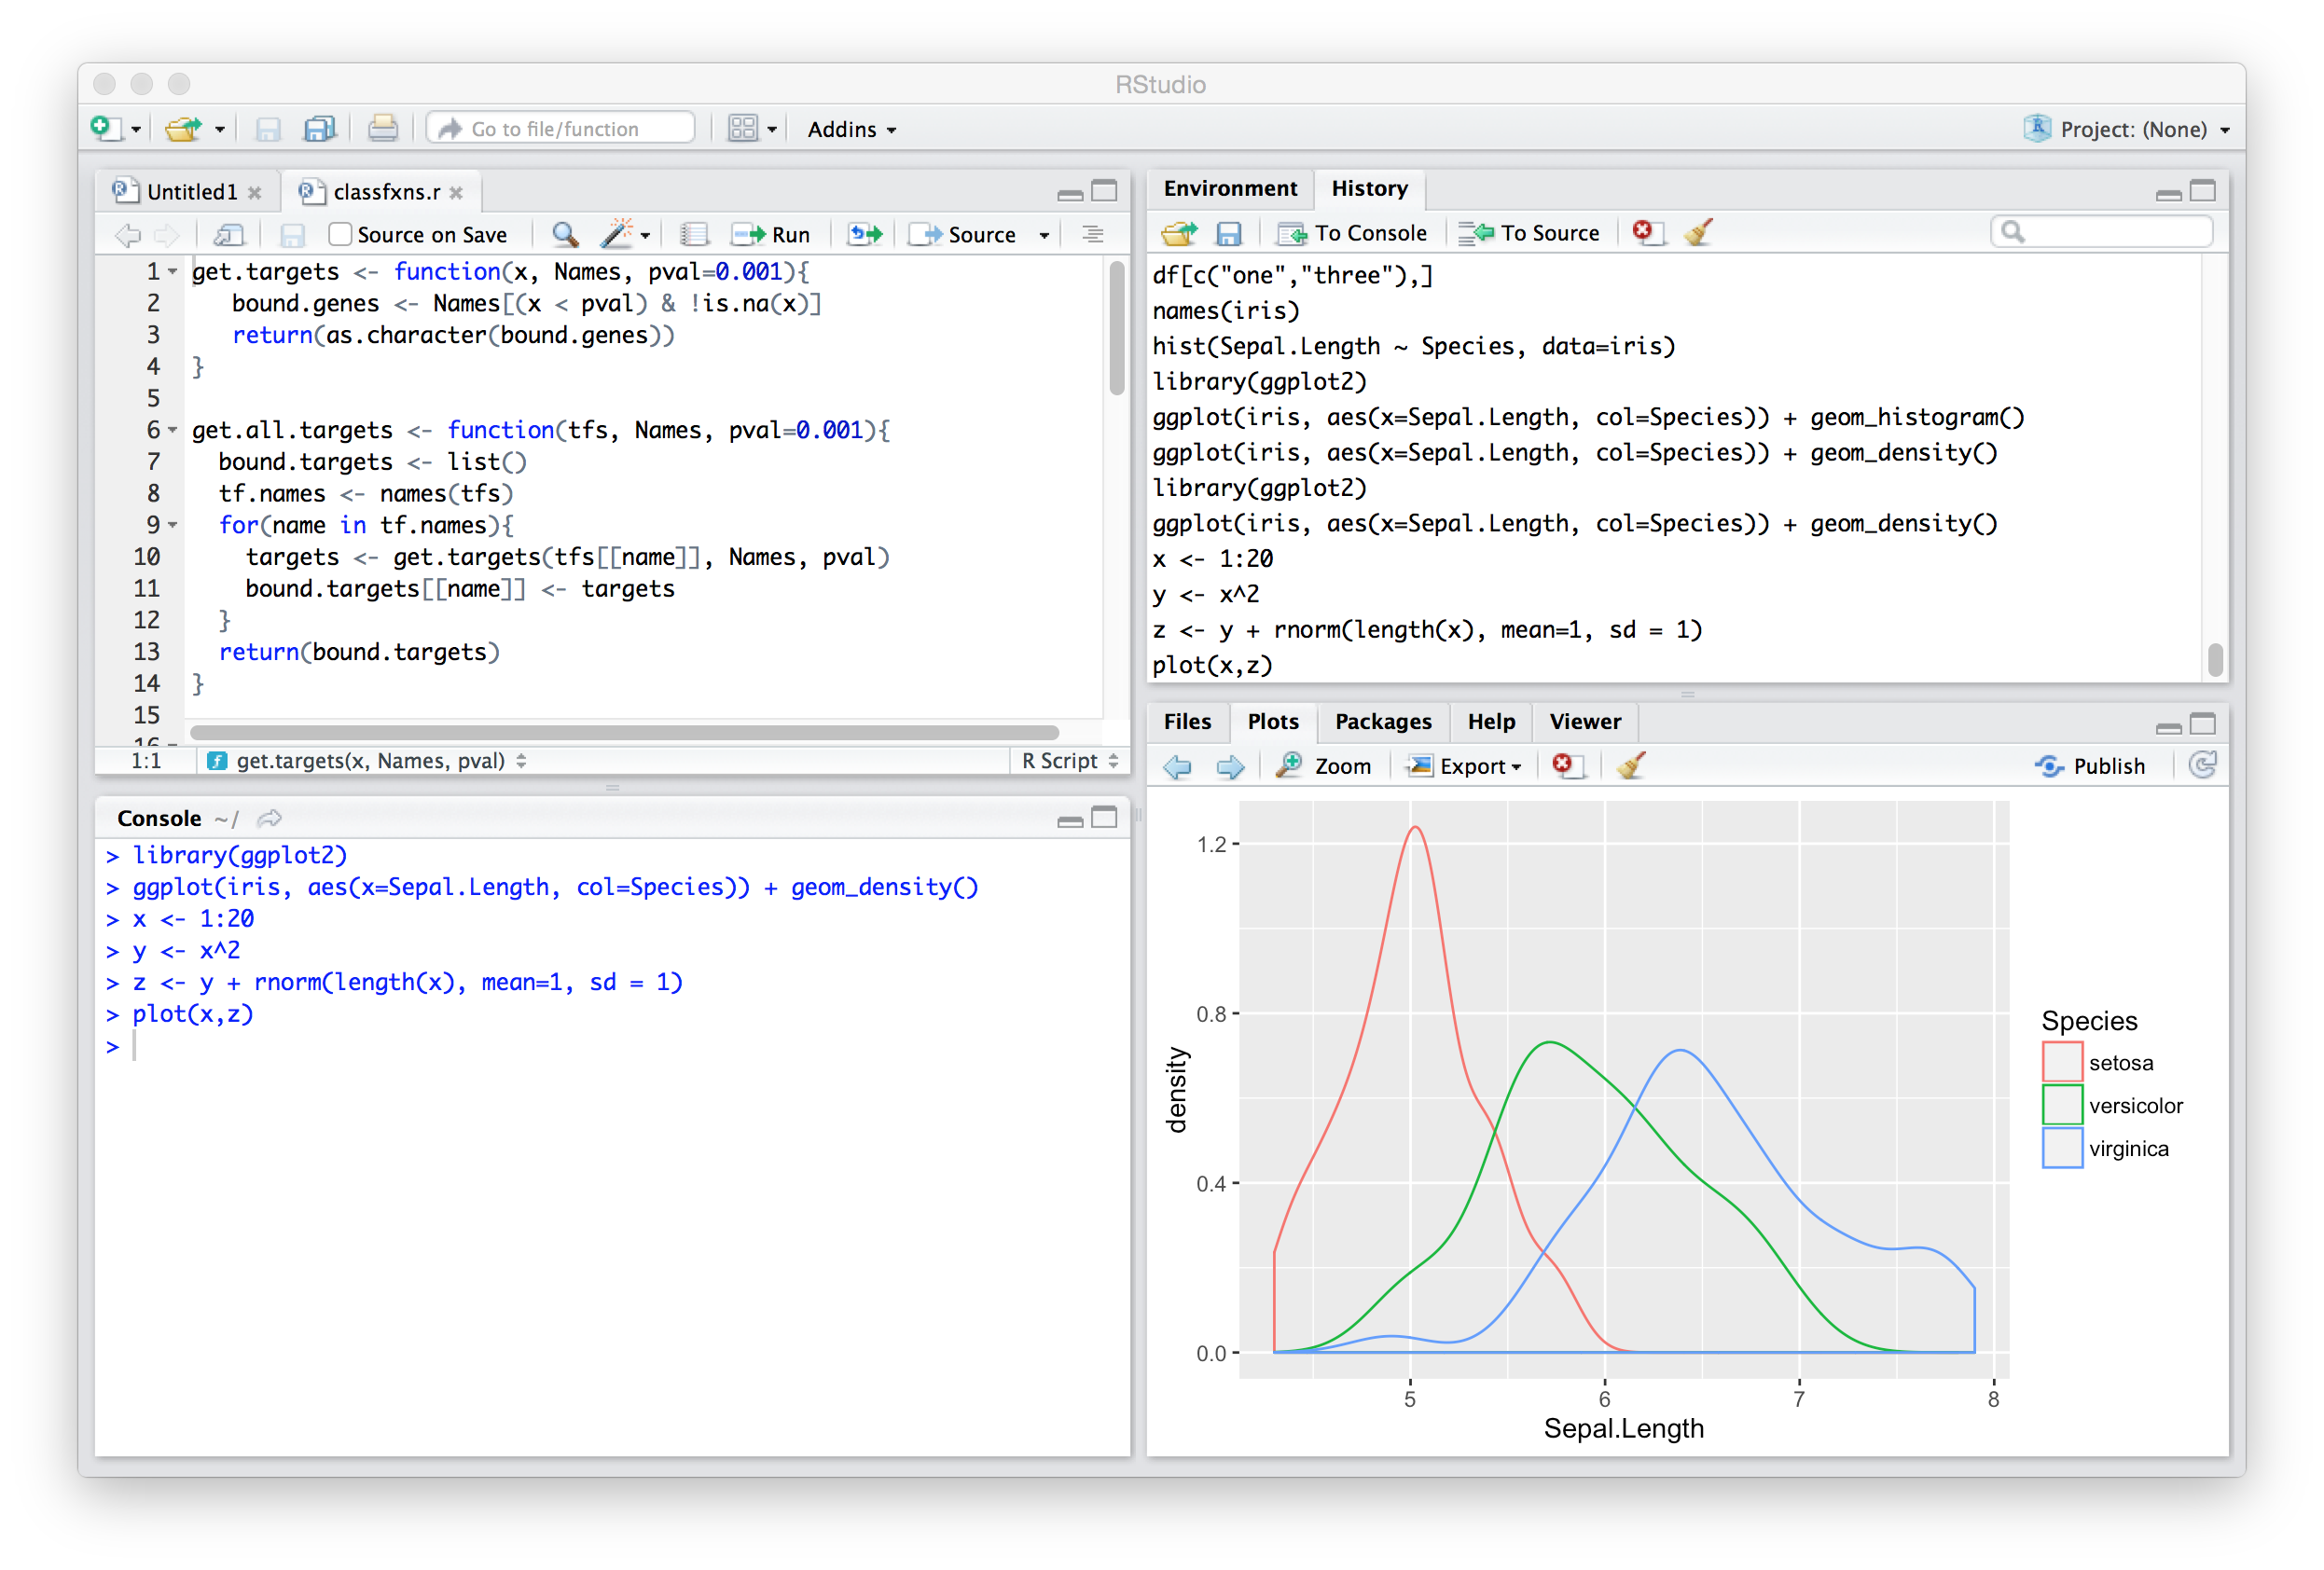
\includegraphics[width=0.9\textwidth]{./rstudio-screen.png}
\caption{The RStudio Environment}
\end{figure}
\end{frame}

\begin{frame}[label={sec:orgheadline5}]{Syllabus, First Third}
\begin{itemize}
\item Getting up to speed with R
\item Data visualization and exploration
\item Quantitative measures for describing univariate and bivariate data
\item Regression and curve fitting
\end{itemize}
\end{frame}

\begin{frame}[label={sec:orgheadline6}]{Syllabus, Second Third}
\begin{itemize}
\item Probability
\item Statistical distributions
\item Understanding sampling distributions of statistics of interest through statistical simulation
\item Central Limit Theorem
\end{itemize}
\end{frame}

\begin{frame}[label={sec:orgheadline7}]{Syllabus, Last Third}
\begin{itemize}
\item Confidence Intervals
\item Hypothesis testing and statistical power
\item \(t\)-tests
\item ANOVA
\item Regression revisited
\item \(\chi^2\) and contingency tables
\end{itemize}
\end{frame}


\begin{frame}[label={sec:orgheadline8}]{Course policies: Academic Integrity}
\begin{itemize}
\item All students are expected to adhere to and have an obligation to act in accordance with the Duke Community Standard.

\item Strict adherence to the plagiarism policy described in the Community Standard will be observed. Any violations of the community standard will be referred to the undergraduate judicial board.

\item Students are encouraged to study together and discuss the course material.
\end{itemize}
\end{frame}


\begin{frame}[label={sec:orgheadline9}]{Course policies: Missed classes}
\begin{itemize}
\item Religious/Athletic/Interviews -- Must notify instructor at least \alert{one week} in advance about missed class time.

\item Illness -- STINF or letter from academic dean if long-term illness.

\item Students with excused absences other than illness are still expected to submit problem sets by assigned dates.
\end{itemize}
\end{frame}

\begin{frame}[label={sec:orgheadline10}]{Grading}
\begin{block}{Quizzes}
In-class quizzes related to readings and lecture material from previous classes. Multiple choice or short answer.
\end{block}

\begin{block}{Problem sets}
Weekly statistical and computational problems based on the material covered in lectures and the readings. 12 assignments total; lowest score dropped.
\end{block}

\begin{block}{Late assignments}
Homework assignments that are submitted late without a STINF or instructor approval will receive half credit if submitted within 24 hours of the due date, or zero credit thereafter.
\end{block}
\end{frame}

\begin{frame}[label={sec:orgheadline11}]{Bonus points for on-time assignment completion}
Students completing all problem sets and quizzes on time, and without any excused absences or STINFs, will receive bonus points towards their final grade.
\end{frame}


\begin{frame}[label={sec:orgheadline12}]{Texts}
\begin{figure}[htb]
\centering

\includegraphics[height=0.75\textheight]{./tufte-cover.png}
\caption{Tufte, 2001. The Visual Display of Quantitative Information.}
\end{figure}
\end{frame}


\begin{frame}[label={sec:orgheadline13}]{Texts}
\begin{figure}[htb]
\centering
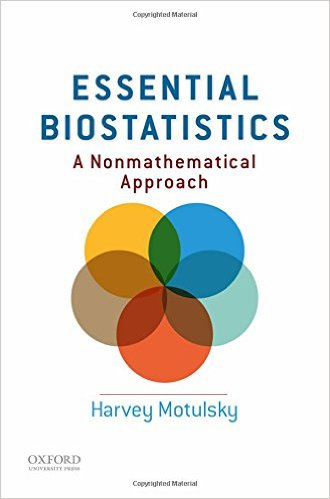
\includegraphics[height=0.75\textheight]{./motulsky-cover.jpg}
\caption{Motulsky, 2015. Essential Biostatistics: A Nonmathematical Approach.}
\end{figure}
\end{frame}


\begin{frame}[label={sec:orgheadline14}]{Texts}
\begin{itemize}
\item \href{http://www.nature.com/collections/qghhqm/pointsofsignificance}{Nature Methods, Points of Significance} -- A series of short articles, published 2013-2015, on key statistical topics, aimed at the working biologist.
\end{itemize}
\end{frame}

\begin{frame}[label={sec:orgheadline15}]{Class materials}
\begin{itemize}
\item Sakai -- submitting problem sets and viewing grades

\item \href{https://github.com/Bio204-class/Bio204-Fall-2016/wiki}{Class wiki} -- everything else. See link in the PDF version of this slide or on Sakai. 
\begin{itemize}
\item Direct link:
\end{itemize}
\url{https://github.com/Bio204-class/Bio204-Fall-2016/wiki}
\end{itemize}
\end{frame}

\begin{frame}[label={sec:orgheadline16}]{In class survey}
Fill out the survey at \url{https://goo.gl/forms/iQiH1ml08JNkMzgA2}
\end{frame}


\begin{frame}[label={sec:orgheadline17}]{Hands-on exercise: Describe a small data set}
See handout
\end{frame}
\end{document}